% 10-30 páginas

\newcommand{\din}[0]{\ensuremath{\delta_{in}}}
\newcommand{\dout}[0]{\ensuremath{\delta_{out}}}
\newcommand{\gin}[0]{\ensuremath{\mathrm{g}_{in}}}
\newcommand{\gout}[0]{\ensuremath{\mathrm{g}_{out}}}

\chapter{Redes Complexas} \label{cap:redes} 

\begin{section}{Introdução} \label{sec:redes-complexas} % Rodrigo: tá muito seco!

% Mais recentemente, grafos têm sido objeto de estudo de um ramo da física estatística denominado teoria das redes complexas. Este capítulo descreve alguns avanços dessa teoria que são relevantes para este trabalho.

A teoria das redes complexas estuda propriedades gerais de diversos tipos de redes, representadas como grafos, com o uso de ferramentas estatísticas. Estudos realizados na última década revelaram similaridades entre redes estudadas em diversos domínios. Exemplos incluem redes tecnológicas, como a Web e a rede de distribuição de energia elétrica dos Estados Unidos, redes biológicas, como cadeias alimentares e redes de ligações entre proteínas, e redes sociais, como as relações de amizade entre alunos de uma escola \cite{Newman2003}.

O termo ``rede'' em geral está associado a entidades reais, como pessoas e relacionamentos de amizade, enquanto o termo ``grafo'' designa uma abstração matemática conveniente para representar relacionamentos entre objetos. Na teoria das redes complexas, no entanto, os termos são frequentemente usados como sinônimos, e é desta forma que eles são usados neste trabalho.

Barabási e Albert \cite{Barabasi1999} analisaram uma amostra da \emph{World Wide Web}, modelada como um grafo não-orientado no qual os vértices representam páginas e as arestas representam \emph{links} entre duas páginas. Eles observaram a distribuição dos graus dos vértices, isto é, o número de vértices conectados a outros $k$ vértices ($N(k)$), para cada valor de $k > 0$, e encontraram uma lei de potência, isto é, acharam $N(k)$ proporcional a $k^{-\gamma}$, como mostra a Figura \ref{fig:leidepotencia}. Desde então, leis de potência têm sido encontradas na distribuição de graus de redes estudadas em diversos domínios, inclusive no domínio de software, com $\gamma$ variando tipicamente entre 2 e 3. Redes com esse padrão são chamadas de \emph{redes livres de escala}.

% Eles perceberam que o número de vértices com grau $k$, isto é, vértices ligados a outros $k$ vértices, era aproximadamente proporcional a $k^{-\gamma}$, função conhecida como lei de potência (veja a Figura \ref{fig:leidepotencia}). Desde então, esse padrão de conectividade tem sido encontrado em redes estudadas em diversos domínios, inclusive no domínio de software. Redes com esse padrão são chamadas de redes \emph{livres de escala}.

% Explicar que não há valor característico para o grau de um vértice, e daí vem o nome.

\begin{figure}[htbp]
	\centering
	\includegraphics[width=0.6\textwidth]{figuras/leidepotencia}
	\caption{Distribuição do número de arestas por vértice do tipo lei de potência. Adaptado de \cite{Barabasi2007}.}
	\label{fig:leidepotencia}
\end{figure}

% No caso de redes orientadas, há duas distribuições a serem consideradas: a distribuição dos graus de entrada e a distribuição dos graus de saída. Nas redes orientadas que são livres de escala, ambas as distribuições seguem leis de potência.

% e alto coeficiente de clustering

Se diversas redes possuem um mesmo padrão de distribuição de graus, o que as diferencia? Milo e outros pesquisadores \cite{Milo2002} estudaram a estrutura de redes orientadas de diversos domínios em busca da resposta. Para isso, eles listaram 13 possíveis configurações de arestas em redes com 3 vértices --- as chamadas tríades ---, mostradas na Figura \ref{fig:triades}. Contando o número de vezes que cada tríade aparece em uma rede, é possível formar um vetor, denominado \emph{perfil de concentração de tríades} (PCT), que é característico de redes de um domínio. 

O papel dos PCTs na caracterização de domínios de redes é ilustrado nas Figuras \ref{fig:tcp}(a) e \ref{fig:tcp}(b). Na primeira Figura, são apresentados PCTs de redes de dois domínios distintos: uma rede de software e uma rede linguística. Na segunda, são apresentados PCTs de duas redes do mesmo domínio, o domínio de software. Uma análise informal dos gráficos revela que a similaridade entre os PCTs é maior no segundo caso, no qual as redes são do mesmo domínio. No primeiro caso, é notável a diferença nas concentrações das duas primeiras tríades (de cima para baixo). 
% 

\begin{figure}[htbp]
	\centering
		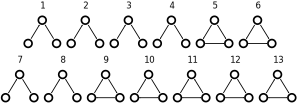
\includegraphics[scale=1]{figuras/triads}
	\caption{Tríades, ou grafos com três vértices, numeradas de 1 a 13.}
	\label{fig:triades}
\end{figure}

\begin{figure}[htbp]
	\centering
		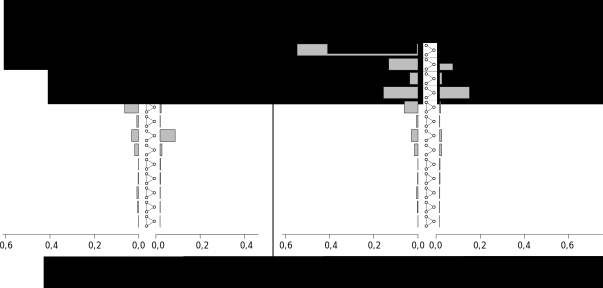
\includegraphics[width=1\textwidth]{figuras/tcp}
	\caption{Comparação entre perfis de concentração de tríades de três redes distintas. (a) À esquerda, rede de dependências entre as classes do programa JabRef, versão 2.5b2; à direita, rede de adjacências entre palavras da língua japonesa \cite{Milo2004}. (b) À esquerda, a rede do programa JabRef, versão 2.5b2; à direita, a rede do programa ArgoUML, versão 0.28.}
	\label{fig:tcp}
\end{figure}

A similaridade entre PCTs pode ser quantificada através do coeficiente de correlação de Pearson entre os PCTs \cite{Milo2004}. O resultado é um valor entre -1 (menor similaridade) e 1 (maior similaridade). Na Figura \ref{fig:tcp}(a), o coeficiente de correlação vale $0,68$; na Figura \ref{fig:tcp}(b), $0,98$. Os números confirmam a análise informal e mostram que a correlação é maior no caso em que as redes pertencem ao mesmo domínio.

Vale notar que o coeficiente de correlação neste caso não possui significado estatístico. Ainda assim, ele tem sido usado de forma bem sucedida na pesquisa de Milo.

A partir da similaridade entre PCTs pode-se construir uma métrica de similaridade entre redes. Sejam $a$ e $b$ duas redes, PCT($x$) o vetor com as concentrações das tríades na rede $x$ e cor($x, y$) o coeficiente de correlação de Pearson entre dois vetores. A similaridade entre as redes, sim($a$, $b$), é dada por

$$
\mathrm{sim}(a, b) ~=~ 
  \mathrm{cor}(\mathrm{PCT}(a), \mathrm{PCT}(b))\mathrm{.}
$$

\end{section}

\begin{section}{Redes de Dependências no Domínio de Software}

	Redes são muito usadas no domínio de engenharia de software para representar as dependências entre entidades do código-fonte, tais como classes em linguagens orientadas a objetos. 
	%
	Estudos recentes têm aplicado a teoria das redes complexas a redes de dependências entre entidades do código-fonte de sistemas de software. 
	%
	(Daqui pra frente, tais redes serão denominadas \emph{redes de software}, em contraste com redes biológicas, redes sociais etc.) Um dos principais resultados é a constatação de que redes de software são livres de escala.
	%
	
	Valverde e Solé \cite{Valverde2003} estudaram redes não-orientadas formadas por relações de agregação de tipos em diagramas UML, programas em C e programas em C++. Myers \cite{Myers2003} analisou redes de chamadas de função em programas em C e redes de agregação e herança em programas em C++. Em ambos os casos as redes foram identificadas como livres de escala. 

	Redes livres de escala também foram encontradas em programas escritos em Smalltalk \cite{Marchesi2004,Concas2007} e em Java \cite{Hyland-Wood2006,Baxter2006,Ichii2008}, em dependências entre pacotes de software \cite{Labelle2004}, em dependências entre bibliotecas dinâmicas \cite{Louridas2008} e até mesmo em referências entre objetos em tempo de execução \cite{Potanin2005}.
\end{section}

\begin{section}{Modelos de Geração de Redes}
% deu 7 páginas
% Organizadas em Módulos

Para tentar explicar os mecanismos responsáveis pela formação de redes livres de escala em diversos domínios, vários modelos de redes livres de escala foram propostos. Os modelos são algoritmos que geram vértices e arestas de forma probabilística porém de acordo com certas regras que garantem que, quando o número de vértices tende a infinito, a distribuição dos graus dos vértices tende a uma lei de potência. Tais modelos, portanto, geram redes similares a redes de software, ao menos quanto à distribuição dos graus.

Assim como um sistema de software é organizado conceitualmente em módulos, uma rede de software deve representar suas entidades organizadas em módulos. A maioria dos modelos de redes livres de escala, no entanto, gera redes sem qualquer tipo de organização hierárquica.

Após uma pesquisa extensa, embora não-sistemática, realizada durante o primeiro semestre de 2009, foram encontrados dois modelos de redes livres de escala organizadas em módulos: o modelo CGW \cite{Chen2008} e o modelo LFR \cite{Lancichinetti2008,Lancichinetti2009}. Um terceiro modelo, o BCR+, elaborado no contexto deste trabalho, é descrito no próximo capítulo.

A seguir são apresentados quatro modelos de redes. Os dois primeiros, o de Erdős–Rényi (ER) e o de Barabási-Albert (BA), geram redes sem módulos, e são apresentados aqui a fim de ilustrar conceitos usados nos outros modelos.
 
% Modelo de Erdos-Renyi?
% Modelo de configuração?
% Modelo de Albert-Barabasi?

\begin{subsection}{O modelo de Erdős–Rényi (ER)}
	O modelo de Erdős–Rényi (ER) \cite{Erdos1959} gera redes não-orientadas nas quais a distribuição dos graus dos vértices tende à distribuição de Poisson . Ele foi concebido antes da teoria das redes complexas. O modelo ER recebe dois parâmetros:
	
	\begin{itemize}
		\item $n$, o número de vértices;
		\item $m$, o número de arestas.
	\end{itemize}
	
	Uma rede com $n$ vértices pode conter até $\frac{n(n-1)}{2}$ arestas. Nas redes geradas pelo modelo ER, $m$ arestas são selecionadas aleatoriamente dentre as arestas potenciais. Cada aresta potencial tem a mesma probabilidade de ser selecionada.
	
	O modelo pode ser adaptado facilmente para gerar redes orientadas. Neste caso, uma rede com $n$ vértices pode conter até $n(n-1)$ arestas, e é desse conjunto de aresta que $m$ vértices são selecionados.
	
	Pela descrição do modelo, percebe-se que ele pode gerar qualquer rede possível, com qualquer distribuição de graus. A probabilidade de uma rede gerada pelo modelo ER ser livre de escala é, no entanto, baixíssima.

\end{subsection}

\begin{subsection}{O modelo de Barabási-Albert (BA)}	
	
	O modelo de Barabási-Albert (BA) \cite{Barabasi1999} foi o primeiro modelo livre de escala da teoria das redes complexas. Ele gera redes não-orientadas, livres de escala e sem módulos através de dois mecanismos: crescimento e ligação preferencial. Crescimento significa que as redes são construída a partir da adição sucessiva de novos vértices. Ligação preferencial significa que os vértices com mais arestas têm mais probabilidade de receber novas arestas.
	
	O modelo BA aceita os seguinte parâmetros:
	
	\begin{itemize}
		\item $n$, o número de vértices da rede final;
		\item $m$, o número de arestas adicionadas a cada passo.
	\end{itemize}
	
	A rede é inicializada com um número arbitrário de vértices e arestas de forma que cada vértice possua grau maior ou igual a 1. A cada passo, é adicionado um novo vértice, que é ligado através de $m$ novas arestas a $m$ vértices pré-existentes. Os $m$ vértices são escolhidos de acordo com a ligação preferencial, o que significa que a probabilidade de um vértice $x$ ser escolhido é proporcional ao grau de $x$: $\mathrm{P}(x) \sim \mathrm{g}(x)$. Como a soma dos probabilidades dos vértices deve ser igual a 1, a probabilidade de cada vértice é igual ao seu grau dividido pela soma dos graus de todos os vértices da rede:
	
	$$
	\mathrm{P}(x) ~=~ \frac{\mathrm{g}(x)}{\sum_y \mathrm{g}(y)},
	$$
	
	onde g($x$) representa o grau do vértice $x$. Diz-se que os novos vértices se conectam \emph{preferencialmente} a vértices com alto grau. Como consequência, alguns poucos vértices acumulam muitas arestas, enquanto a maioria dos vértices com permanece com poucas arestas. O processo é repetido até que a rede atinja $n$ vértices.
	
	% TODO: IMPORTANTE %% A Figura XXX exemplifica o mecanismo de ligação preferencial.
	
	% MELHOR DEIXAR ISSO DE FORA: Várias adaptações já foram propostas para o modelo BA. Uma adaptação simples pode ser realizada para que o modelo gere redes orientadas. No caso de redes orientadas, as $m$ arestas orientadas adicionadas a cada passo possuem origem no novo vértice. O mecanismo de ligação preferencial pode levar em conta os graus totais dos vértices, $\mathrm{g}(x)$, ou apenas os graus de entrada, $\gin(x)$.

\end{subsection}

\begin{subsection}{O modelo CGW}

O modelo CGW \cite{Chen2008} gera redes orientadas, livres de escala e organizadas em módulos. Baseado no modelo BA, ele utiliza os mecanismos de crescimento e ligação preferencial. Ele foi proposto como um modelo da evolução de sistemas de software. O modelo aceita 11 parâmetros:

\begin{itemize}
\item número de vértices, $n$;
\item número de módulos, $m$;
\item quatro probabilidades, $p_1, p_2, p_3, p_4$, com $p_1 + p_2 + p_3 + p_4 = 1$ e $p_1 > 0$;
\item quatro números naturais, $e_1, e_2, e_3, e_4$;
\item uma constante, $\alpha$, com $\alpha \ge -1$.
\end{itemize}

Nesse modelo, a construção inicia-se com uma rede inicial arbitrária e então vai crescendo de acordo com determinadas regras de formação, até alcançar $n$ vértices. Cada vértice é atribuído a exatamente um dos $m$ módulos no momento em que é criado.

A rede inicial é alterada pela aplicação sucessiva de quatro regras em ordem aleatória:

\begin{itemize}
	
	\item Regra 1: com probabilidade $p_1$, um novo vértice é adicionado a um módulo escolhido aleatoriamente, juntamente com $e_1$ arestas com origem no novo vértice. Os vértices de destino das $e_1$ arestas são escolhidos de acordo com a probabilidade preferencial baseada em módulos (PPBM), explicada mais à frente.
	
	\item Regra 2: com probabilidade $p_2$, são adicionadas $e_2$ arestas. Para cada aresta, o vértice de origem é escolhido aleatoriamente, enquanto o vértice de destino é escolhido de acordo com a PPBM.
	
	\item Regra 3: com probabilidade $p_3$, $e_3$ arestas são religadas. O procedimento de religamento de arestas é descrito a seguir:
	
	\begin{enumerate}
		\item um vértice, $v_1$ é escolhido aleatoriamente;
		\item uma aresta, $a_1$, escolhida aleatoriamente dentre as arestas com origem em $v_1$, é removida da rede;
		\item é adicionada uma nova aresta cuja origem é $v_1$ e o vértice de destino é escolhido de acordo com a PPBM;
	\end{enumerate}
	
	\item Regra 4: com probabilidade $p_4$, $e_4$ arestas escolhidas aleatoriamente são removidas da rede.
	
\end{itemize}

Naturalmente, as probabilidades $p_1, p_2, p_3$ e $p_4$ devem somar 1. Além disso, $p_1$ deve ser maior que zero --- do contrário o número de vértices na rede permanece constante. As quantidades $e_1, e_2, e_3, $ e $e_4$ são inteiros maiores ou iguais a zero.

A probabilidade preferencial baseada em módulos, $\Pi(v_2|v_1)$, é uma função que indica a probabilidade de se escolher um vértice, $v_2$, como destino de uma aresta cujo vértice de origem, $v_1$, já foi determinado. O propósito da PPBM é controlar a proporção de arestas externas na rede, privilegiando a escolha de um vértice de destino pertencente ao mesmo módulo do vértice de origem (ou pertence a outro módulo, a depender do valor de $\alpha$). Eis a definição da probabilidade preferencial baseada em módulos:

$$
\Pi (v_2|v_1) ~=~
\left\{
\begin{array}{cl}
\dfrac{1 + \mathrm{g}(v_2) \cdot (1 + \alpha)}{Q(v_1)} 
  & \mbox{se $v_2$ está no mesmo módulo de $v_1$} \vspace{0.5em} \\ 
\dfrac{1 + \mathrm{g}(v_2)}{Q(v_1)} 
  & \mbox{caso contrário}
\end{array}
\right.
$$

O parâmetro $\alpha$ controla a proporção de arestas externas na rede. Para $\alpha = -1$, a maioria das arestas serão externas. Para $\alpha > 0$, a maioria das arestas serão internas, e quanto maior o valor de $\alpha$, maior a tendência. Quando $\alpha = 0$, arestas internas e externas são igualmente prováveis.

A expressão g($v$) designa o grau de saída do vértice $v$. O termo $Q$ é apenas uma constante de proporcionalidade cujo propósito é fazer a soma das probabilidades ser igual a 1, e é definido da seguinte forma:

$$
Q(v_1) = \sum_{v \in m(v_1)} (1 + \mathrm{g}(v) \cdot (1 + \alpha))
~+ \sum_{v \notin m(v_1)} (1 + \mathrm{g}(v))
$$

A expressão m($v$), neste contexto, designa o conjunto dos vértices que pertencem ao mesmo módulo de $v$.

\end{subsection}

\begin{subsection}{O modelo LFR}

O modelo LFR \cite{Lancichinetti2008,Lancichinetti2009} é um modelo flexível que pode gerar redes com arestas ponderadas e módulos sobrepostos, isto é, nas quais um vértice pode pertencer a mais de um módulo. Diferentemente do CGW, o LFR não é um modelo de crescimento: todos os vértices são gerados de uma vez e então são adicionadas as arestas.

Nesta pesquisa foi estudado um caso particular do modelo no qual todas as arestas têm o mesmo peso e os módulos não se sobrepõem. Foi usada a implementação original dos autores, disponível em  \url{http://santo.fortunato.googlepages.com/inthepress2}. O modelo aceita os seguintes parâmetros:

\begin{itemize}
\item número de vértices, $n$;
\item grau de entrada médio, $k$, com $k < n$;
\item grau de entrada máximo, $max_k$, com $k \le max_k < n$;
\item parâmetro de mistura, $\mu$, com $0 \le \mu \le 1$;
\item expoente da distribuição de graus, $-\gamma$;
\item expoente da distribuição de tamanho de módulos, $-\beta$;
\item tamanho do menor módulo, $min_m$;
\end{itemize}

Os tamanhos dos módulos são selecionados de uma lei de potência com expoente $-\beta$. O parâmetro de mistura, $\mu$, é a proporção de arestas externas na rede gerada. No modelo LFR, nem todas as combinações de parâmetros são factíveis. Por exemplo, se $n = 100$, então $min_m$ não pode ser 60, caso contrário existiriam módulos menores do que $min_m$.

	%A geração da rede é feita através de um processo iterativo com rápida convergência.
	
	% ﰊ1ﰋ Each node is given a degree taken from a power law distribution with exponent ﰃ. The extremes of the distribu- tion kmin and kmax are chosen such that the average degree is ﰎkﰏ. The configuration model ﰌ18ﰍ is used to connect the nodes so to keep their degree sequence.
	% ﰊ2ﰋ Each node shares a fraction 1−ﰅ of its links with the other nodes of its community and a fraction ﰅ with the other nodes of the network; ﰅ is the mixing parameter.
	% ﰊ3ﰋ The sizes of the communities are taken from a power law distribution with exponent ﰄ, such that the sum of all sizes equals the number N of nodes of the graph. The mini- mal and maximal community sizes smin and smax are chosen so to respect the constraints imposed by our definition of community: sminﰆkmin and smaxﰆkmax. This ensures that a node of any degree can be included in at least a community.
	% ﰊ4ﰋ At the beginning, all nodes are homeless, i.e., they are not assigned to any community. In the first iteration, a node is assigned to a randomly chosen community; if the commu- nity size exceeds the internal degree of the node ﰊi.e., the number of its neighbors inside the communityﰋ, the node enters the community, otherwise it remains homeless. In suc- cessive iterations we place a homeless node to a randomly chosen community: if the latter is complete, we kick out a randomly selected node of the community, which becomes homeless. The procedure stops when there are no more homeless nodes.
	% ﰊ5ﰋ To enforce the condition on the fraction of internal neighbors expressed by the mixing parameter ﰅ, several re- wiring steps are performed, such that the degrees of all nodes stay the same and only the split between internal and exter- nal degree is affected, when needed. In this way the ratio between external and internal degree of each node in its com- munity can be set to the desired share ﰅ with good approxi- mation ﰊsee Fig. 1ﰋ.

\end{subsection}

\end{section}

\begin{section}{Conclusão} % síntese, súmula, resumo
	
	A teoria das redes complexas é uma área de pesquisa madura, que oferece ferramentas teóricas que apoiam o estudo de redes do ponto de vista estatístico. A teoria tem sido aplicada com sucesso no estudo de diversos domínios, como a sociologia, a biologia e a engenharia.
	
	Redes livres de escala são redes que possuem uma determinada distribuição de graus. Redes de dependências entre entidades de software já foram identificadas como redes livres de escala em diversos estudos recentes.
	
	Perfis de concentração de tríades (PCTs) caracterizam redes através de vetores de treze números. Eles podem ser usados para medir a similaridade estrutural entre duas redes.
	
	CGW e LFR são modelos que geram redes livres de escala organizadas em módulos. Com tais propriedades, essas redes podem representar dependências entre entidades de software.
	
\end{section}

% == O modelo BCR ==
% 
% O modelo BCR gera redes livres de escala orientadas e sem módulos. Assim como o modelo BA, ele adota os mecanismos de crescimento e ligação preferencial. O modelo BCR aceita os seguintes parâmetros:
% 
% \begin{itemize}
% 	\item três probabilidades, $p_1$, $p_2$ e $p_3$, tal que $p_1 + p_2 + p_3 = 1$;
% 	\item dois números reais, $\din$ e $\dout$.
% \end{itemize}
% 
% A partir de uma rede inicial, a cada passo é aplicado uma operação, escolhida dentre três operações de acordo com as probabilidades $p_1$, $p_2$ e $p_3$:
% 
% \begin{itemize}
% 	\item Com probabilidade $p_1$, é adicionado um novo vértice, $v$, juntamente com uma aresta de $v$ até um vértice pré-existente, $w$. O vértice $w$ é escolhido de acordo com $g_{in}(x) + \din$, onde $g_{in}$ representa o grau de entrada. Isso significa que a probabilidade de um vértice arbitrário ($x$) ser escolhido é proporcional a $g_{in}(x) + \din$ --- ou seja, $mathrm{P}(x) = \frac{g_{in}(x) + \din}{\sum_y g_{in}(y) + \din}$.
% 	
% 	\item Com probabilidade $p_2$, é adicionado um novo vértice, $w$, juntamente com uma aresta de um vértice pré-existente, $v$, até $w$. O vértice $w$ é escolhido de acordo com $g_{out} + \dout$, onde $g_{out}$ representa o grau de saída.
% 	
% 	\item Com probabilidade $p_3$, é adicionada uma aresta de um vértice pré-existente, $v$, até outro vértice pré-existente, $w$. O vértice $v$ é escolhido de acordo com $g_{out} + \dout$, onde $g_{out}$. O vértice $w$ é escolhido de acordo com $g_{out} + \dout$.
% \end{itemize}
